\documentclass[12pt]{beamer}
\usepackage{beamerthemeHannover, graphicx, clrscode, amsmath, amssymb, multicol}
\usepackage{verbatim}

\setbeamercolor{sidebar}{use=structure,bg=gray!20!green!60!white}
\title{Scientific Computing With Perl and Math::GSL}
\author[J.A. Leto]{Jonathan Leto - jonathan@leto.net}
\date{}

\begin{document}
\begin{frame}[t]
        \titlepage
        \begin{center}
        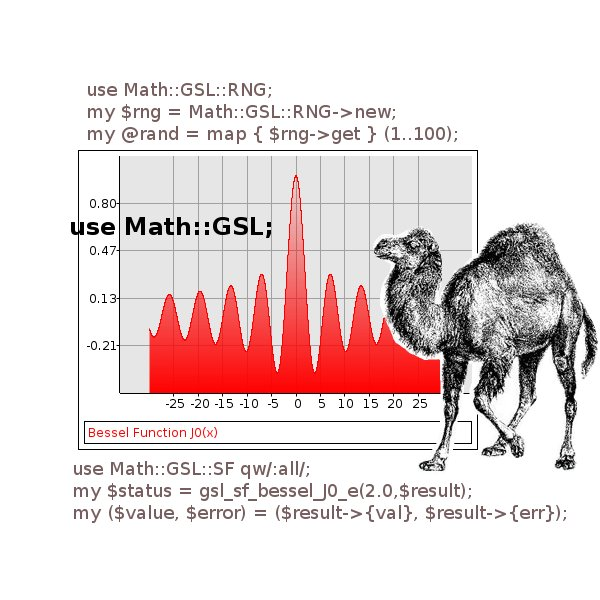
\includegraphics[width=4.50cm, height=4.50cm]{perl_sci}
        \end{center}
\end{frame}

\section{Why do "Science" with Perl?}
\frame{
    \frametitle{Why do "Science" with Perl?}
    \begin{center}
    \begin{itemize}
        \item Minimize development time
        \item CPAN 
        \item Data Munging 
        \item Camels are cool, FORTRAN isn't
    \end{itemize}
    \end{center}
}

\section{Basic Tools}
\frame{
    \frametitle{Basic Tools}
    \begin{center}
    \begin{itemize}
        \item PDL - Perl Data Language
            \begin{itemize}
                \item Basic datatype is an N-dimensional matrix of numbers
                \item Very fast
                \item Low level
                \item Overwhelming for a beginner
            \end{itemize}
        \item Math::GSL - Interface to the GNU Scientific Library
            \begin{itemize}
                \item 422 special functions, hundreds of statistical distributions, descriptive statics,
                        random and quasi-random number generators, FFT, numerical derivative/integration, etc...
                \item Very fast
                \item Needs more syntax sugar
            \end{itemize}
    \end{itemize}
    \end{center}
}

\section{Math::GSL Examples}
\begin{frame}[fragile]
    \frametitle{Random Number Generators}
    Math::GSL currently has support for 64 different random number generators.
    \begin{center}
    \begin{small}
    \begin{verbatim}
    my $rng  = Math::GSL::RNG->new;
    my @nums = map { $rng->get } (1 .. 1000);
    \end{verbatim}

    \begin{verbatim}
    my $rng  = Math::GSL::RNG
                ->new($gsl_rng_knuthran, 31337);
    while ( my $num = $rng->get ){
        ...
    }
    \end{verbatim}
    \end{small}
    \end{center}
\end{frame}

\begin{frame}[fragile]
    \frametitle{Vectors and Matrices}
    \begin{center}
    \begin{small}
    \begin{verbatim}
    my $v = Math::GSL::Vector->new([1 .. 10]);
    my $w = Math::GSL::Vector->new([10 .. 1]);
    my $dot_product = $v * $w;
    my $scaled_v = 5 * $v;
    my ($min,$max) = ($v->min,$v->max);

    \end{verbatim}

    \begin{verbatim}
    my $matrix  = Math::GSL::Matrix->new(5,5);
    $matrix->set_col(0, [1 .. 5 ])
           ->set_row(2, [6 .. 10]);
    my $first_row = $matrix->row(0);
    print "First row is: " . 
        join(' ',$first_row->as_list) . "\n";

    \end{verbatim}
    \end{small}
    \end{center}
\end{frame}

\begin{frame}[fragile]
    \frametitle{But really, what's inside?}
    \begin{tiny}
    Math::GSL::BLAS           
    Math::GSL::BSpline         
    Math::GSL::CBLAS           
    Math::GSL::CDF           
    \colorbox{red}{Math::GSL::Chebyshev     } 
    Math::GSL::Combination     
    \colorbox{yellow}{Math::GSL::Complex} 
    Math::GSL::Const           
    Math::GSL::DHT             
    \colorbox{yellow}{Math::GSL::Deriv           }
    Math::GSL::Eigen           
    Math::GSL::Errno           
    \colorbox{yellow}{Math::GSL::FFT            } 
    \colorbox{yellow}{Math::GSL::Fit            } 
    \colorbox{red}{Math::GSL::Heapsort       } 
    Math::GSL::Histogram       
    \colorbox{red}{Math::GSL::Histogram2D     }
    \colorbox{yellow}{Math::GSL::Integration    } 
    \colorbox{yellow}{Math::GSL::Interp         } 
    Math::GSL::Linalg          
    Math::GSL::Machine         
    Math::GSL::Matrix          
    \colorbox{yellow}{Math::GSL::Min            } 
    \colorbox{red}{Math::GSL::Monte           }
    \colorbox{red}{Math::GSL::Multifit        }
    \colorbox{red}{Math::GSL::Multimin        }
    \colorbox{red}{Math::GSL::Multiroots      }
    Math::GSL::NTuple          
    \colorbox{red}{Math::GSL::ODEIV}
    Math::GSL::Permutation     
    Math::GSL::Poly            
    Math::GSL::PowInt          
    Math::GSL::QRNG 
    Math::GSL::RNG             
    Math::GSL::Randist         
    \colorbox{yellow}{Math::GSL::Roots            }
    Math::GSL::SF               
    \colorbox{red}{Math::GSL::Siman           } 
    Math::GSL::Sort             
    \colorbox{yellow}{Math::GSL::Spline           }
    Math::GSL::Statistics       
    \colorbox{yellow}{Math::GSL::Sum             } 
    Math::GSL::Sys              
    Math::GSL::Vector           
    Math::GSL::Wavelet          
    \colorbox{red}{Math::GSL::Wavelet2D      }  
    \end{tiny}

\end{frame}

\section{Going Forward}
\frame{
    \frametitle{Scientific Computing Environment}
    \begin{itemize}
        \item Computer Algebra System - gsl\_repl and Math::*
        \item Numerics - Math::GSL and PDL
        \item Visualization - Cairo, Chart::Clicker, ?
        \item Data Assistant - ?
    \end{itemize}
}
\frame{
    \frametitle{Active Development Continues}

    \begin{itemize}
        \item Scientific Computing applications built on top of Math::GSL
        \item Math::Symbolic integration
        \item PDL integration
        \item Callbacks and threaded Perls
    \end{itemize}
}
\section{Acknowledgements}
\frame{
    \frametitle{Thanks}

    \begin{itemize}
        \item Eric Wilhelm
        \item Thierry Moisan
        \item \#pdx.pm
    \end{itemize}
}

\frame{
    \frametitle{More Info}
    \begin{itemize}
        \item {http://leto.net/gitweb/}\\
        \item {http://leto.net/code/Math-GSL/}\\
        \item {http://groups.google.com/group/math-gsl-dev}\\
        \item {http://groups.google.com/group/perl-scientific-computing}\\
    \end{itemize}
}

\end{document}
